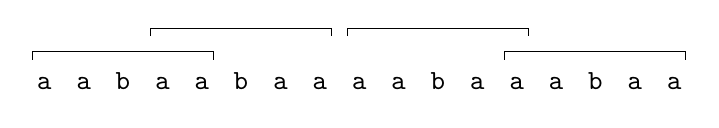
\begin{tikzpicture}[xscale=0.5]
  \foreach \x/\c in {
    1/a,2/a,3/b,4/a,5/a,
    6/b,7/a,8/a,
    9/a,10/a,11/b,12/a,13/a,
    14/a,15/b,16/a,17/a
  }  \draw (\x,0) node[above] {\tt \c};
  \draw[yshift=-0.4cm] (0.7,0.9) -- (0.7,1) -- (5.3,1) -- (5.3,0.9);
  \draw[xshift=3cm,yshift=-0.1cm] (0.7,0.9) -- (0.7,1) -- (5.3,1) -- (5.3,0.9);
  \draw[xshift=8cm,yshift=-0.1cm] (0.7,0.9) -- (0.7,1) -- (5.3,1) -- (5.3,0.9);
  \draw[xshift=12cm,yshift=-0.4cm] (0.7,0.9) -- (0.7,1) -- (5.3,1) -- (5.3,0.9);
\end{tikzpicture}
